% !TeX root = RJwrapper.tex 
\title{A Computational Analysis of the Dynamics of R Style Based on 94 Million Lines of Code from All CRAN Packages in the Past 20 Years}
\author{by Chia-Yi Yen, Mia Huai-Wen Chang, Chung-hong Chan}

\maketitle

\abstract{
There are so many programming style variations in R. We have analyzed 94 million lines of R code and quantified the evolution in popularity of 12 style-elements from 1998 to 2018. We attribute 3 main factors that drive changes in programming style: effect of style-guides, effect of introducing new features, and effect of editors. A consensus in programming style is forming and we have summarised it into a consensus-based style.
}

\section{Introduction}

R is flexible. For example, one can use \code{<-} or \code{=} as assignment operators. The following two functions can both be correctly evaluated.

\begin{example}
sum_of_square <- function(x) {
    return(sum(x^2))
}
\end{example}

\begin{example}
sum_of_square = function(x) {
    return(sum(x ^ 2))
}
\end{example}

One area that can highlight this flexible is naming conventions. According to the previous research by \citet{baaaath}, there are at least 6 styles and none of the 6 has dominated the scene. There are still some other style-elements that R programmers have the freedom to adopt, e.g. whether or not to add spaces around infix operators, use double quotation marks or single quotation marks to denote strings, etc. On one hand, these variations provide programmers with freedom. On the other hand, these variations can confuse new programmers and can have dire effects on program comprehension. Also, incompatibility between programming styles might also affect reuse, maintainability \citep{elish} and open source collaboration \citep{wang}. 

Various efforts to standardize the programming style, e.g. Google's R Style Guide \citep{google}, The Tidyverse Style Guide \citep{tidyverse}, Bioconductor Coding Style \citep{bioconductor} etc.,  are available (Table~\ref{tab:table1}). These style guides are based on the normative assessment of code quality, e.g. style-elements that improve program comprehension \citep{oman}. However, we argue that one should first study the current situation, and preferably, the historical development, of programming style variations (PSV) to supplement these standardization efforts. We have undertaken such a task, so that the larger R community can have a baseline to evaluate the effectiveness of those standardization efforts. Also, we can have a better understanding of the factors driving increase and decrease in PSV historically, such that more effective efforts can be formulated.

\newcolumntype{L}{>{\centering\arraybackslash}m{3cm}}

\begin{table}

\caption{\label{tab:table1}Three major style-guides: Google, Tidyverse and Bioconductor}
\centering
\begin{tabular}[t]{L|L|L|L}
\hline
Feature & Google & Tidyverse & Bioconductor\\
\hline
Function name & UpperCamel & snake\_case & lowerCamel\\
\hline
Assignment & Discourage = & Discourage = & Discourage =\\
\hline
Line length & “limit your code to 80 characters per line” & “limit your code to 80 characters per line” & $\leqslant$ 80\\
\hline
Space after a comma & Yes & Yes & Yes\\
\hline
Space around infix operators & Yes & Yes & Yes\\
\hline
Indentation & 2 spaces & 2 spaces & 4 spaces\\
\hline
Quotes & Double & Double & Not specified\\
\hline
Boolean values & Use TRUE / FALSE & Use TRUE / FALSE & Not specified\\
\hline
Terminate a line with a semicolon & No & No & Not specified\\
\hline
Curly braces & \{ same line, then a newline, \} on its own line & \{ same line, then a newline, \} on its own line & Not specified\\
\hline
\end{tabular}
\end{table}


\section{Analysis}
\subsection{Data Source}

In January 2019, we cloned a local mirror of CRAN using the rsync method suggested in the CRAN Mirror HOWTO \citep{cranminihowto}. In our local mirror, it contains all packages as tarball files (.tar.gz). By all packages, we mean packages actively listed online on the CRAN websites and packages delisted for whatever reasons e.g. no maintainer, etc. In this analysis, we include all packages, i.e. including those delisted.

In order to facilitate the analysis, we have developed the \code{baaugwo} package to extract all R source code and metadata from these tarballs. In this study, only the source code from the \code{/R} directory of each tarball file is included. We have also archived the metadata from the \code{DESCRIPTION} and \code{NAMESPACE} files from the tarballs.

In order to cancel out the over-representation effect of multiple submissions in a year by a particular package, we have applied the \emph{"one-submission-per-year"} rule to randomly selected only one submission from a year for each package. Unless explicitly notice, we present below the analysis of this \emph{"one-submission-per-year"} sample. Similarly, unless explicitly notice, the unit of the analysis is \emph{exported function}. The study period for this study is from 1998 to 2018.

\subsection{Quantification of PSV}

Every exported function in our sample are parsed into a parse tree using the parser from the \CRANpkg{lintr} \citep{lintr} package.

These parse trees were then filtered for lines with function definition and then linted them using the linters from the lintr package to detect for various style-elements. Style-elements considered in this study are:

\paragraph{fx\_assign}

Use = as assignment operators

\begin{example}
softplusFunc = function(value, leaky = FALSE) {
    if (leaky) {
        warnings("using leaky RELU!")
        return(ifelse(value > 0L, value, value * 0.01))
    }
    return(log(1L + exp(value)))
}
\end{example}

\paragraph{fx\_opencurly}

An open curly is on its own line

\begin{example}
softplusFunc <- function(value, leaky = FALSE) 
{
    if (leaky) 
    {
        warnings("using leaky RELU!")
        return(ifelse(value > 0L, value, value * 0.01))
    }
    return(log(1L + exp(value)))
}
\end{example}

\paragraph{fx\_infix}

No spaces are added around infix operators.

\begin{example}
softplusFunc<-function(value, leaky=FALSE) {
    if (leaky) {
        warnings("using leaky RELU!")
        return(ifelse(value>0L, value, value*0.01))
    }
    return(log(1L+exp(value)))
}
\end{example}

\paragraph{fx\_integer}

Not explicitly type integers

\begin{example}
softplusFunc <- function(value, leaky = FALSE) {
    if (leaky) {
        warnings("using leaky RELU!")
        return(ifelse(value > 0, value, value * 0.01))
    }
    return(log(1 + exp(value)))
}
\end{example}

\paragraph{fx\_singleq}

Use single quotation marks for strings

\begin{example}
softplusFunc <- function(value, leaky = FALSE) {
    if (leaky) {
        warnings('using leaky RELU!')
        return(ifelse(value > 0L, value, value * 0.01))
    }
    return(log(1L + exp(value)))
}
\end{example}

\paragraph{fx\_commas}

No space is added after commas

\begin{example}
softplusFunc <- function(value,leaky = FALSE) {
    if (leaky) {
        warnings("using leaky RELU!")
        return(ifelse(value > 0L,value,value * 0.01))
    }
    return(log(1L + exp(value)))
}
\end{example}

\paragraph{fx\_semi}

Use semicolons to terminate lines

\begin{example}
softplusFunc <- function(value, leaky = FALSE) {
    if (leaky) {
        warnings("using leaky RELU!");
        return(ifelse(value > 0L, value, value * 0.01));
    }
    return(log(1L + exp(value)));
}
\end{example}

\paragraph{fx\_t\_f}

Use T/F instead of TRUE / FALSE

\begin{example}
softplusFunc <- function(value, leaky = F) {
    if (leaky) {
        warnings("using leaky RELU!")
        return(ifelse(value > 0L, value, value * 0.01))
    }
    return(log(1L + exp(value)))
}
\end{example}

\paragraph{fx\_closecurly}

An close curly is not on its own line.

\begin{example}
softplusFunc <- function(value, leaky = FALSE) {
    if (leaky) {
        warnings("using leaky RELU!")
        return(ifelse(value > 0L, value, value * 0.01)) }
    return(log(1L + exp(value))) }
\end{example}

\paragraph{fx\_tab}

Use tab to indent

\begin{example}
softplusFunc <- function(value, leaky = FALSE) {
    if (leaky) {
        warnings("using leaky RELU!")
        return(ifelse(value > 0L, value, value * 0.01))
    }
    return(log(1L + exp(value)))
}
\end{example}

We have studied also the naming conventions of all included functions. Using the similar technique of \citet{baaaath}, we classified function names into the following 7 categories:

\begin{itemize}
  \item \textbf{alllower} softplusfunc
  \item \textbf{ALLUPPER} SOFTPLUSFUNC
  \item \textbf{UpperCamel} SoftPlusFunc
  \item \textbf{lowerCamel} softPlusFunc
  \item \textbf{lower\_snake} soft\_plus\_func
  \item \textbf{dotted.func} soft.plus.func
  \item \textbf{other} sOfTPluSfunc
\end{itemize}

The last style-element is line-length. For each R file, we counted the distribution of line-length. In this analysis, the unit of analysis is line.

By not considering line-length, we have studied 10 binary style-elements and one multinomial style-element with 7 categories. Therefore, the possible number of combinations based on these 11 style-elements is: $7 \times 2^{10} = 7168$.

\subsection{Community-specific variations}

On top of the overall patterns based on the analysis of all functions, the community-specific variations are also studied. In this part of the study, we ask the question: do local patterns of PSV exist in various programming communities? To this end, we constructed a dependency graph of CRAN packages by defining a package as a node and an import/suggest relationship as a directed edge. Communities in this dependency graph were extracted using the Walktrap Community Detection Algorithm \citep{pons} provided by the \CRANpkg{igraph} package \citep{csardi}. The step parameter was set at 4 for this analysis. Notably, we analyzed the dependency graph as a snapshot, which is built based on the latest submission of each package in or before 2018.

The 18 largest communities were extracted to study local patterns in PSV.

\section{Results}

We studied more than 94 million lines of code from 15530 unique packages. In total, 1898142 exported functions were studied. Figure~\ref{figure:fig1} displays the popularity of the 10 binary style-elements from 1998 to 2008. Some style-elements have very clear trends towards a majority-vs-minority pattern, e.g. fx\_closecurly, fx\_semi, fx\_t\_f and fx\_tab. Some styles-elements are instead trending towards a divergence from a previous majority-vs-minority pattern, e.g. fx\_assign, fx\_commas, fx\_infix, fx\_integer, fx\_opencurly and fx\_singleq. There are two style-elements that deserve special scrutiny. Firstly, the variation in fx\_assign is a clear example illustrating the effect of introducing a new language element by the R Development Core Team. The introduction of the language feature (= as assignment operator) in R 1.4 \citep{chambers} has coincided with the taking off in popularity of such style-element since 2001. Up to now, around 20\% of exported functions use such style.

\begin{figure}[htbp]
  \centering
  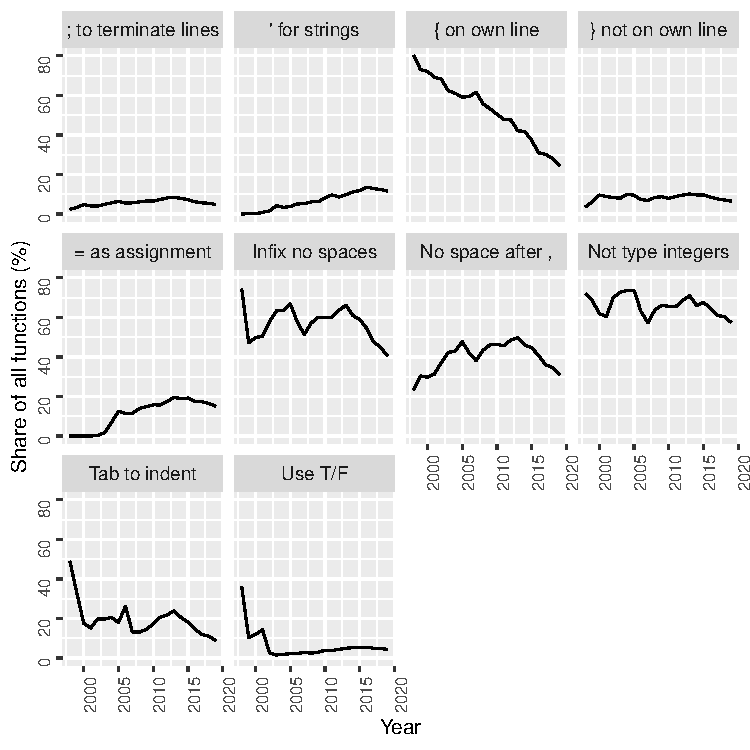
\includegraphics{fig1}
  \caption{Evolution in popularity of 10 style-elements from 1998 to 2018.}
  \label{figure:fig1}
\end{figure}


Secondly, the popularity of fx\_opencurly shows how a previously established majority style (~80\% in late 90s) slowly reduced into a minority but still very prominent style (~30\% in late 10s).

Similarly, the evolution of different naming conventions is shown in Figure~\ref{figure:fig1}. This analysis can best be used to illustrate the effect of style-guides. According to \citet{baaaath}, dotted.func style is very specific to R programming. This style is the most dominant style in the early days of CRAN. However, multiple style guides advise against the use of dotted.func style and thus a significant declining trend is observed. lower\_snake and UpperCamel are the styles endorsed by the Tidyverse Style Guide and the Google's R Style Guide respectively. These two styles see an increasing trend since the 10s, although the growth of lower\_snake is relatively more impressive. To our surprise, lowerCamel case, a style endorsed by Bioconductor, is currently the most popular naming convention (22.5\% in 2018). However, its reign might soon be dethroned by lower\_snake (21.5\% in 2018) in the near future.


\begin{figure}[htbp]
  \centering
  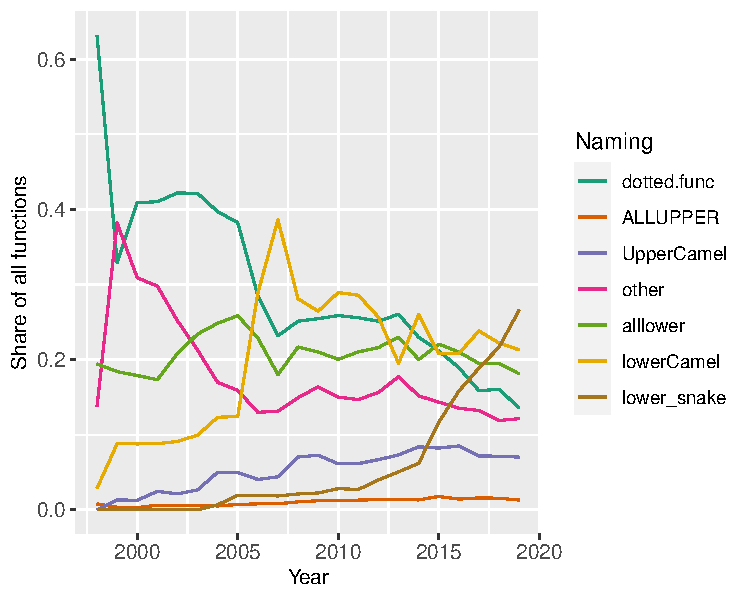
\includegraphics{fig2}
  \caption{Evolution in popularity of 7 naming conventions from 1998 to 2018.}
  \label{figure:fig2}
\end{figure}

The evolution of line lengths is tricky to be visualized on a 2-D surface. We have prepared an animation (\url{https://github.com/chainsawriot/rstyle/blob/master/file60f331694ef5.gif}) to visualize the change in line distribution over the span of 20 years. In this paper, Figure~\ref{figure:fig3} shows the snapshot of the change in line length distribution in the range of 40 characters to 100 characters. In general, developers of newer packages write with a lesser number of characters per line. Similar to previous analyses with Python programs (e.g. \citet{vanderplas}), artificial peaks corresponding to recommendations from either style-guides, linters, and editor settings are also observed in our analysis. In 2018, the artificial peak of 80 characters (recommended by most of the style-guides and linters such as \CRANpkg{lintr} is more pronounced for lines with comments but not those with actual code.


\begin{figure}[htbp]
  \centering
  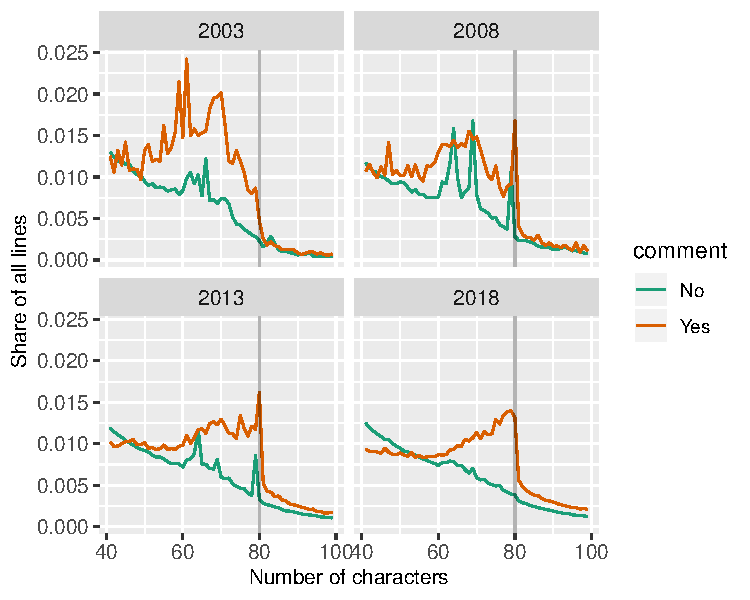
\includegraphics{fig3}
  \caption{Change in line length distribution: 2003, 2008, 2013 and 2018.}
  \label{figure:fig3}
\end{figure}


\subsection{Community-based variations}

Using the aforementioned community detection algorithm of the dependency graph, 18 large communities were extracted. These communities are named by their applications. Table~\ref{tab:table2} lists the details of these communities.

Using the naming convention as an example, there are local patterns in PSV (Figure~\ref{figure:fig4}). For example, snake case is the most popular naming convention in the "RStudio-related" community as expected because it is the naming convention endorsed by the Tidyverse Style-guide. However, none of the functions exported by the packages from "Time, Date, and Money" community uses such convention.

\begin{table}

\caption{\label{tab:table2}The largest 18 communities and their top 3 packages according to eigenvector centrality}
\centering
\begin{tabular}[t]{l|r|l}
\hline
Community & Number of Packages & Top 3 Packages\\
\hline
RStudio-related & 3426 & knitr, testthat, rmarkdown\\
\hline
base & 2618 & methods, graphics, lattice\\
\hline
Image Plotting & 2228 & png, rgl, highr\\
\hline
RCpp & 677 & Rcpp, inline, pkgKitten\\
\hline
GPS and Geography & 530 & deldir, sp, maptools\\
\hline
Machine learning & 319 & rpart, nnet, randomForest\\
\hline
Text Analysis & 92 & stopwords, NISTunits, ISOcodes\\
\hline
Social Network Analysis & 53 & texreg, network, ergm\\
\hline
Graphics & 49 & apt, BioIDMapper, Blaunet\\
\hline
Graph data structure & 48 & graph, scagnostics, RBGL\\
\hline
Genetics & 44 & AhoCorasickTrie, BinQuasi, biofiles\\
\hline
Finance & 36 & RUnit, RcppCCTZ, CFL\\
\hline
Insurance and Actuary & 34 & rsp, babar, BALD\\
\hline
Numerical Optimization & 30 & pbivnorm, rgenoud, Matching\\
\hline
Sparse Matrix & 30 & registry, slam, Rsymphony\\
\hline
Java & 28 & rJava, RWekajars, AWR\\
\hline
Neuroscience & 27 & STAR, rstream, extremefit\\
\hline
Time, Date, and Money & 27 & tis, setRNG, CDNmoney\\
\hline
\end{tabular}
\end{table}

\begin{figure}[htbp]
  \centering
  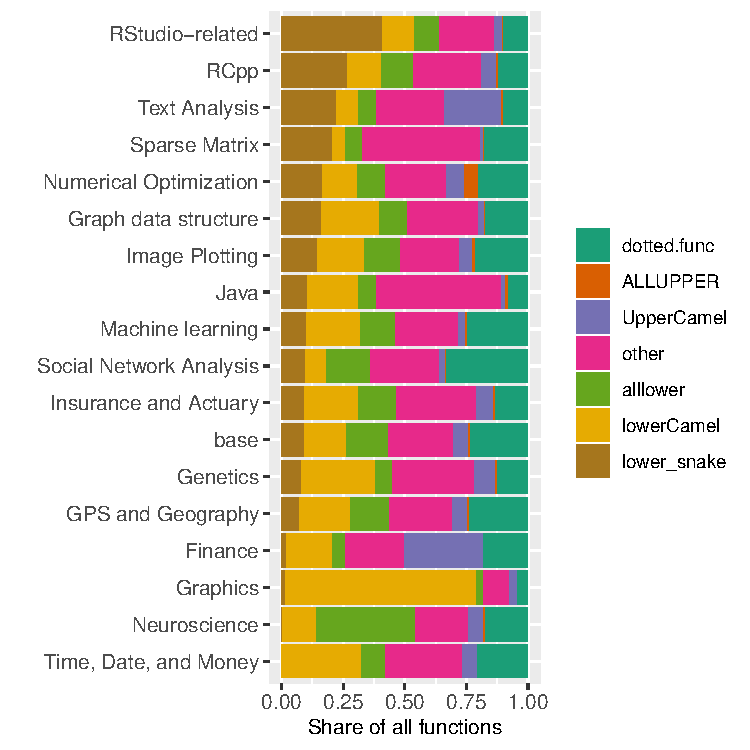
\includegraphics{fig4}
  \caption{Community-specific distribution of naming conventions among 18 large communities.}
  \label{figure:fig4}
\end{figure}

For the binary style-elements, local patterns are also observed (Figure~\ref{figure:fig5}). The most salient pattern is the "Java" and "Sparse Matrix" communities exceptional high usage of tab indentation, probably due to influences from Java or Matlab. Also, the high level in usage of open curly on its own line for the "Graphics" is also exceptional.

\begin{figure}[htbp]
  \centering
  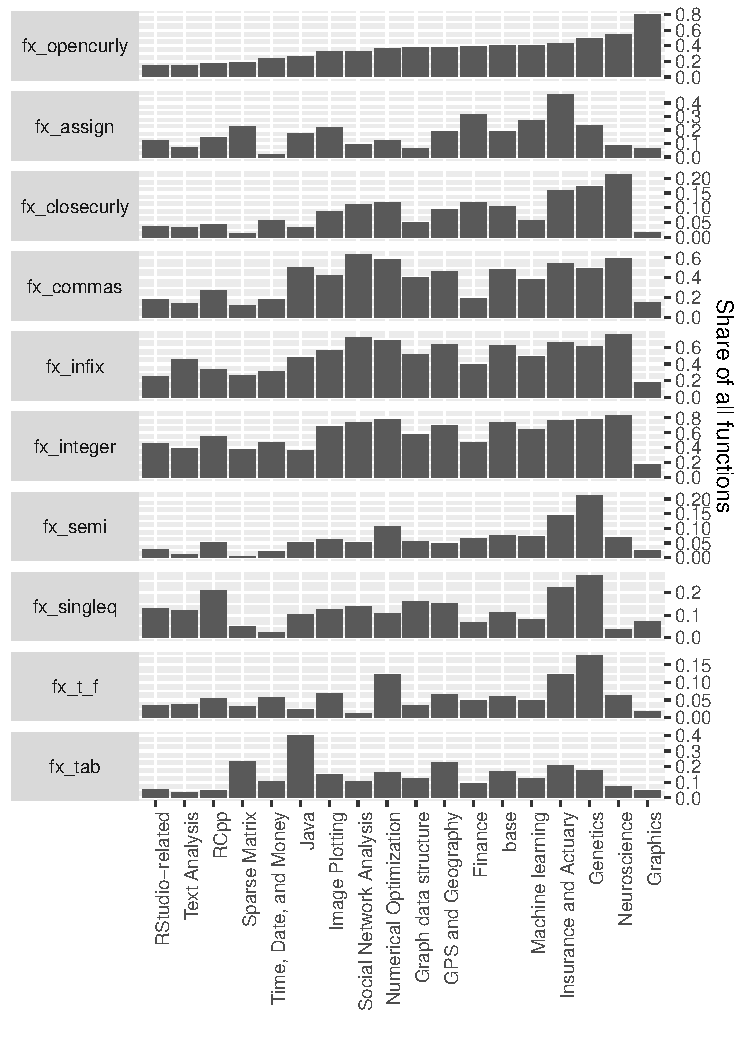
\includegraphics{fig5}
  \caption{Community-specific distribution of style-elements among 18 large communities}
  \label{figure:fig5}
\end{figure}

\section{Discussion}

In this study, we study the PSV in 20 years of CRAN packages across two dimensions: 1) temporal dimension: the longitudinal changes in popularity of various style-elements over 20 years, and 2) cross-sectional dimension: the variations among communities of the latest snapshot of all packages. From our analysis, we identify three factors that possibly drive PSV: effect of style-guides (trending of naming conventions endorsed by \citet{tidyverse} and \citet{google}), the effect of introducing a new language feature (trending of = usage as assignments after 2001) and effect of editors (the dominance of 80-character line limit).

From a policy recommendation standpoint, our study provides important insight for the R Development Core Team and other stakeholders to improve the current situation of PSV in R. Firstly, the introduction of a new language can have a very long-lasting effect on PSV. "Assignments with the = operator" is a feature that introduced by the R Development Core Team to ``increase compatibility with S-Plus (as well as with C, Java, and many other languages).'' \citep{chambers} This might be a good intention but it has an unintended consequence of introducing a very persistent PSV that two major style-guides, \citet{tidyverse} and \citet{google}, consider as a bad style.

Secondly, style-guides, linters, and editors are important standardizers of PSV. Nonetheless, we observe very strong path dependency in programming styles. As indicated by the local patterns of PSV we found in some communities, some package developers are very resistant to these standardizers and keep using their own styles. Having said so, we are not accusing those developers of not following the trendy programming styles. Instead, they follow the mantra of ``if it ain't broke don't fix it''. Again, from a policy recommendation standpoint, the existence of local PSV patterns suggests there are many blind spots to the previous efforts in addressing PSV. Style-guide's authors may consider community outreach to promote their endorsed styles, if they want other communities to adopt their styles.

Our analysis also opens up an open question: should R adopt an official style-guide akin the PEP-8 of the Python Software Foundation \citep{vanrossum}? There are of course pros and cons of adopting such official style-guide. As written by \citet{christiansen}, ``style can easily become a religious issue.'' It is not our intention to meddle in this ``religious issue''. If such an effort would be undertaken by someone else, we suggest the following style. We must stress here that this \emph{consensus-based} style is only the most popular style based on our analysis, i.e. the \emph{Zeitgeist} (the spirit of the age). We have no guarantee that this style can improve clarity or comprehensibility. The following is an example of a function written in such consensus-based style.

\begin{example}
softplusFunc <- function(value, leaky = FALSE) {
    if (leaky) {
        warnings("using leaky RELU!")
        return(ifelse(value > 0, value, value * 0.01))
    }
    return(log(1 + exp(value)))
}
\end{example}

In essense,

\begin{itemize}
  \item Use lowerCamel or snake case
  \item Use <- to assign, don't use =
  \item Add a space after commas
  \item Use TRUE / FALSE, don't use T / F
  \item Put open curly bracket on same line then a newline
  \item Use double quotation mark for strings
  \item Add spaces around infix operators
  \item Don't terminate lines with semicolon
  \item Don’t explicitly type integers (i.e. 1L)
  \item Put close curly bracket on its own line
  \item Don't use tab to indent
\end{itemize}

As a final remark: although enforcing a consistent style can improve open source collaboration \citep{wang}, one must also bear in mind that these rules might need to be adjusted sometimes to cater for programmers with special needs. For example, using spaces instead of tabs for indentation can make code not accessible to visually impaired programmers \citep{mosal}.

\section{Reproducibility}

The data and scripts to reproduce the analysis in this paper are available at \url{https://github.com/chainsawriot/rstyle}.

\bibliography{RJreferences}

\address{Chia-Yi Yen\\
  Mannheim Business School, Universit\"at Mannheim\\
  L 5, 6, 68131 Mannheim\\
  Germany\\
  \url{https://orcid.org/0000-0003-1209-7789}\\
  \email{yen.chiayi@gmail.com}}

\address{Mia Huai-Wen Chang\\
  Akelius Residential Property AB\\
  Erkelenzdamm 11-13, 10999 Berlin\\
  Germany\\
  \email{mia5419@gmail.com}}

\address{Chung-hong Chan\\
  Mannheimer Zentrum f\"ur Europ\"aische Sozialforschung, Universit\"at Mannheim\\
  A5, 6,  68159 Mannheim\\
  Germany\\
  \url{https://orcid.org/0000-0002-6232-7530}\\
  \email{chung-hong.chan@mzes.uni-mannheim.de}}
